\documentclass{article}\usepackage[]{graphicx}\usepackage[]{color}
%% maxwidth is the original width if it is less than linewidth
%% otherwise use linewidth (to make sure the graphics do not exceed the margin)
\makeatletter
\def\maxwidth{ %
  \ifdim\Gin@nat@width>\linewidth
    \linewidth
  \else
    \Gin@nat@width
  \fi
}
\makeatother

\definecolor{fgcolor}{rgb}{0.345, 0.345, 0.345}
\newcommand{\hlnum}[1]{\textcolor[rgb]{0.686,0.059,0.569}{#1}}%
\newcommand{\hlstr}[1]{\textcolor[rgb]{0.192,0.494,0.8}{#1}}%
\newcommand{\hlcom}[1]{\textcolor[rgb]{0.678,0.584,0.686}{\textit{#1}}}%
\newcommand{\hlopt}[1]{\textcolor[rgb]{0,0,0}{#1}}%
\newcommand{\hlstd}[1]{\textcolor[rgb]{0.345,0.345,0.345}{#1}}%
\newcommand{\hlkwa}[1]{\textcolor[rgb]{0.161,0.373,0.58}{\textbf{#1}}}%
\newcommand{\hlkwb}[1]{\textcolor[rgb]{0.69,0.353,0.396}{#1}}%
\newcommand{\hlkwc}[1]{\textcolor[rgb]{0.333,0.667,0.333}{#1}}%
\newcommand{\hlkwd}[1]{\textcolor[rgb]{0.737,0.353,0.396}{\textbf{#1}}}%
\let\hlipl\hlkwb

\usepackage{framed}
\makeatletter
\newenvironment{kframe}{%
 \def\at@end@of@kframe{}%
 \ifinner\ifhmode%
  \def\at@end@of@kframe{\end{minipage}}%
  \begin{minipage}{\columnwidth}%
 \fi\fi%
 \def\FrameCommand##1{\hskip\@totalleftmargin \hskip-\fboxsep
 \colorbox{shadecolor}{##1}\hskip-\fboxsep
     % There is no \\@totalrightmargin, so:
     \hskip-\linewidth \hskip-\@totalleftmargin \hskip\columnwidth}%
 \MakeFramed {\advance\hsize-\width
   \@totalleftmargin\z@ \linewidth\hsize
   \@setminipage}}%
 {\par\unskip\endMakeFramed%
 \at@end@of@kframe}
\makeatother

\definecolor{shadecolor}{rgb}{.97, .97, .97}
\definecolor{messagecolor}{rgb}{0, 0, 0}
\definecolor{warningcolor}{rgb}{1, 0, 1}
\definecolor{errorcolor}{rgb}{1, 0, 0}
\newenvironment{knitrout}{}{} % an empty environment to be redefined in TeX

\usepackage{alltt}

\usepackage{fancyhdr} % Required for custom headers
\usepackage{lastpage} % Required to determine the last page for the footer
\usepackage{extramarks} % Required for headers and footers
\usepackage{graphicx} % Required to insert images
\usepackage{hyperref}
\usepackage{amsmath} %for binomial pdf
\usepackage{parskip} % so that there's space bw paragraphs
\usepackage{float}
\usepackage{amsfonts}

% Margins
\topmargin=-0.45in
\evensidemargin=0in
\oddsidemargin=0in
\textwidth=6.5in
\textheight=9.0in
\headsep=0.25in 

\linespread{1.1} % Line spacing

% Set up the header and footer
\pagestyle{fancy}
\lhead{STAT 534: Spatial} % Top left header
\chead{HW 4} % Top center header
\rhead{Andrea Mack} % Top right header
\lfoot{02/10/2017} % Bottom left footer
\cfoot{} % Bottom center footer
\rfoot{Page\ \thepage\ of\ \pageref{LastPage}} % Bottom right footer
\renewcommand\headrulewidth{0.4pt} % Size of the header rule
\renewcommand\footrulewidth{0.4pt} % Size of the footer rule

\setlength\parindent{0pt} % Removes all indentation from paragraphs
\setlength\parskip{0.5cm}
\restylefloat{table}

%----------------------------------------------------------------------------------------
%	DOCUMENT STRUCTURE COMMANDS
%	Skip this unless you know what you're doing
%----------------------------------------------------------------------------------------

% Header and footer for when a page split occurs within a problem environment
\newcommand{\enterProblemHeader}[1]{
\nobreak\extramarks{#1}{#1 continued on next page\ldots}\nobreak
\nobreak\extramarks{#1 (continued)}{#1 continued on next page\ldots}\nobreak
}

% Header and footer for when a page split occurs between problem environments
\newcommand{\exitProblemHeader}[1]{
\nobreak\extramarks{#1 (continued)}{#1 continued on next page\ldots}\nobreak
\nobreak\extramarks{#1}{}\nobreak
}


%----------------------------------------------------------------------------------------%
\IfFileExists{upquote.sty}{\usepackage{upquote}}{}
\begin{document}



\begin{enumerate}
\item %1
{\it For $\lambda$ = 30 generate 9 realizations of CSR on the unit square. For each realization, construct a kernel estimate of $\lambda$(s). How do the estimated intensity functions compare to the constant intensity under CSR? What precautions does this exercise suggest with regard to interpreting estimates of intensity from a single realization (or data set)? The following R code will simultaneously produce the data and plots.}

{\texttt par(mfrow=c(3,3))
  for(i in 1:9) plot(density(rpoispp(30)))}
{\it Provide me with the images.}

In four of the nine intensity functions created under CSR, there appears to be clear clusters, shown by the yellow ``hot spots". Under CSR, we would not expect to see the clusters, and so the fact that these were created under CSR is concerning because a single realization under CSR may in fact violate CSR. Therefore, testing a null hypothesis of CSR using a single realization could lead to inaccurate conclusions. The inaccurate conclusions could happen many ways. If the true intensity function should be clustered, but the one CSR intensity function used to test is quite clustered, we would fail to reject CSR when we should have. If the true intensity function is CSR but the one CSR intensity function used to test the null hypothesis of CSR looks quite clustered, we may wrongly reject CSR.

\begin{knitrout}\footnotesize
\definecolor{shadecolor}{rgb}{0.969, 0.969, 0.969}\color{fgcolor}

{\centering 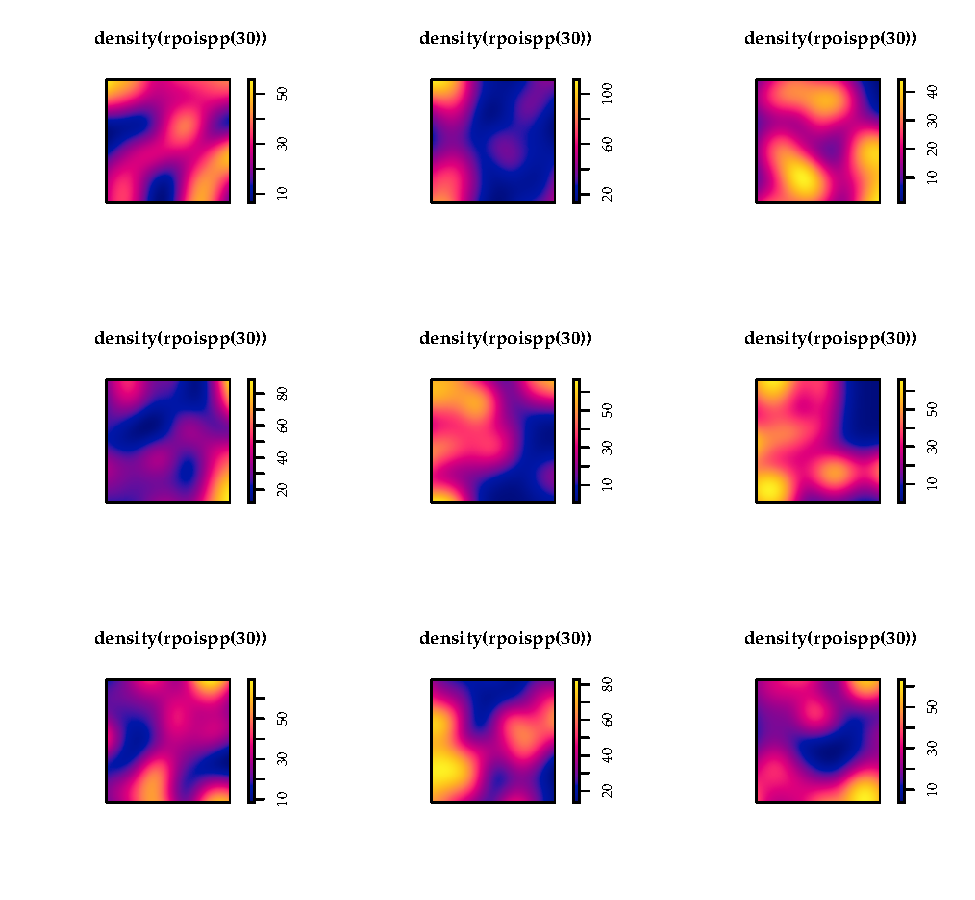
\includegraphics[width=\maxwidth]{figure/prob1-1} 

}



\end{knitrout}



\item %2
{\it In class we looked at a heterogeneous Poisson process on the unit square with with intensity function:}

\begin{center}
$\lambda(x,u) = exp(5x + 2y)$
\end{center}

\begin{enumerate}
\item %2a 
{\it Simulate a realization of the process using the following R code.}

%\texttt{sim.dat$\<$-rpoispp(function(x,y)exp(5*x + 2*y)}

{\it Plot the results and comment.}

The intensity is highest in the upper right corner, near (1,1), and lowest when x ranges from 0 to 0.4 and y ranges from 0 to 1. The locations of the points do not look random.

\begin{knitrout}\footnotesize
\definecolor{shadecolor}{rgb}{0.969, 0.969, 0.969}\color{fgcolor}

{\centering 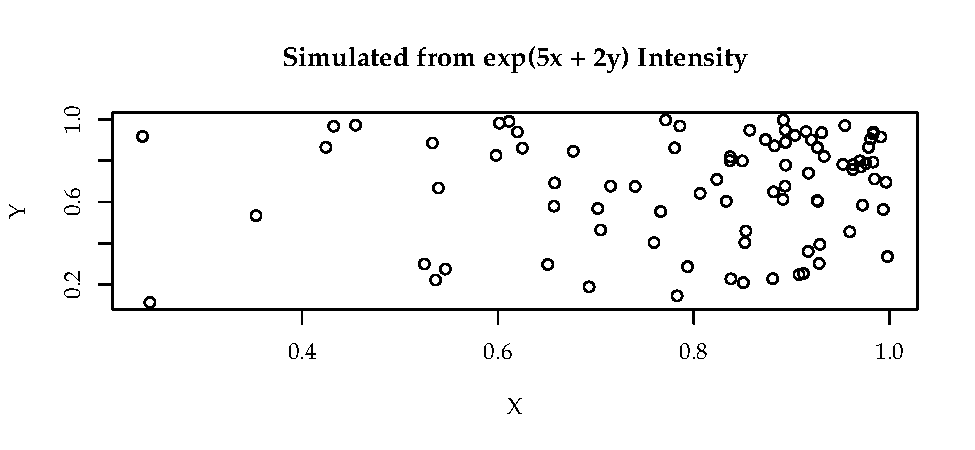
\includegraphics[width=\maxwidth]{figure/prob2a-1} 

}



\end{knitrout}


\newpage

\item %2b
{\it Plot simulation envelopes for the K function (or some suitable modification of it) and comment.}

The plot below suggests strong evidence of clustering as hat(K(r)) - r is above the simulation envelope.

\begin{knitrout}\footnotesize
\definecolor{shadecolor}{rgb}{0.969, 0.969, 0.969}\color{fgcolor}

{\centering 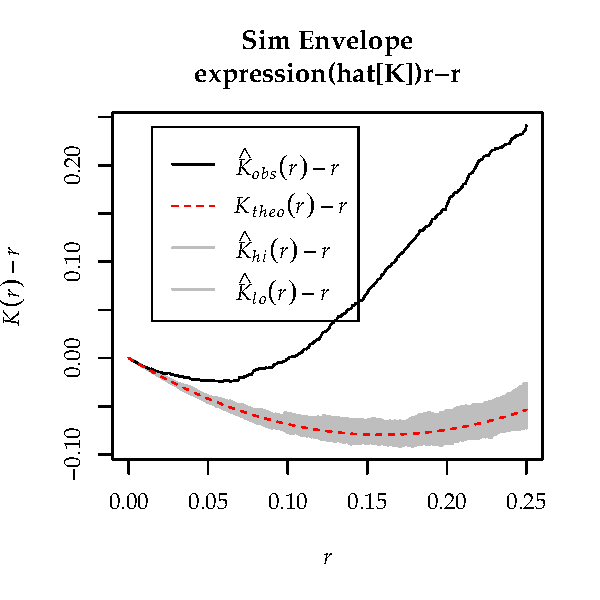
\includegraphics[width=\maxwidth]{figure/prob2b-1} 

}



\end{knitrout}

\item %2c
{\it Fit a trend model to your data using ppm. Provide me with the parameter estimates and associated standard errors.}

% latex table generated in R 3.3.2 by xtable 1.8-2 package
% Fri Feb 10 11:14:45 2017
\begin{table}[ht]
\centering
\begin{tabular}{||l|l|l||}
  \hline
 & Estimate & S.E. \\ 
  \hline
1 & -0.17 & 0.56 \\ 
  2 & 4.89 & 0.58 \\ 
  3 & 2.24 & 0.42 \\ 
   \hline
\end{tabular}
\end{table}


ppm response is log(lambda) and explanatory variables are coordinates

Section: Lilihood methods for fitting models of spatially varying intensity surfaces -- steve thinks this is neat

\item %2d
{\it Check the fit using quadrat.test. Use method=``MonteCarlo" instead of the large sample chi-squared test. Plot the results Discuss.}

With a p-value of 0.56, there is no evidence against CSR after accounting for the heterogenetiy in the intensity parameter across the region.

The largest discrepancies appear to be along the far right column when using the 5X5 grid, however, using Pearson's residual as a measure of the discrepancy between observed and expected show quite low discrepancies despite the seemingly large absolute difference in that column between observed and expected. 


\begin{knitrout}\footnotesize
\definecolor{shadecolor}{rgb}{0.969, 0.969, 0.969}\color{fgcolor}

{\centering 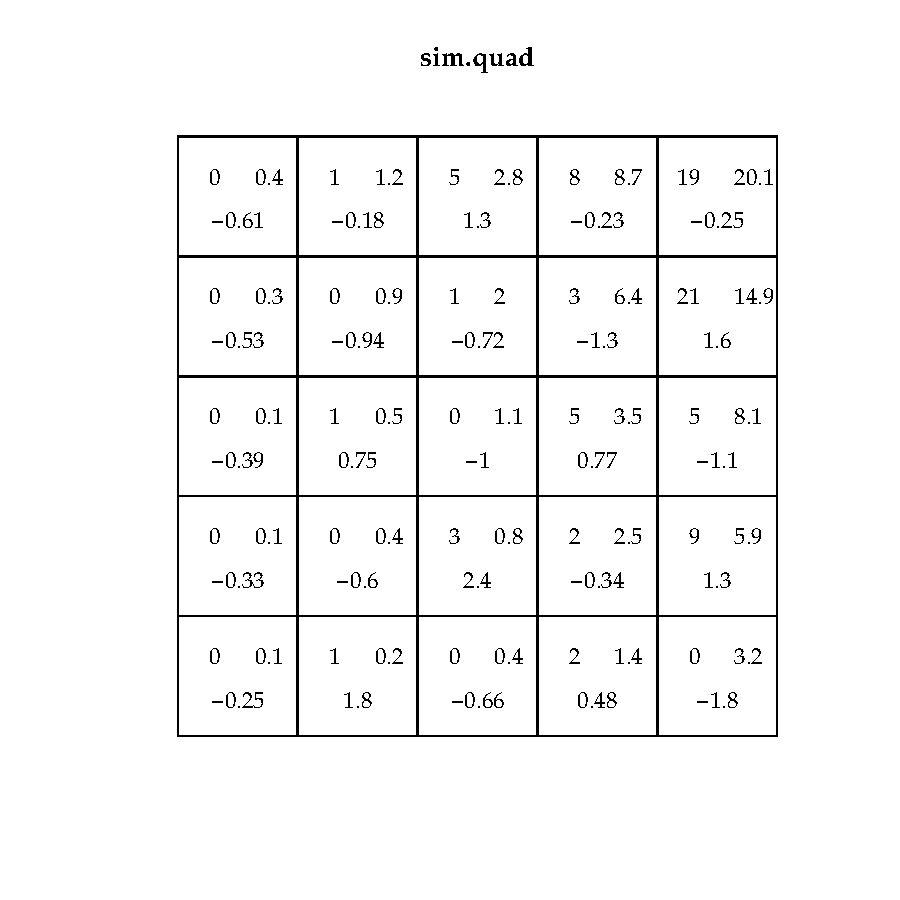
\includegraphics[width=\maxwidth]{figure/prob2d-1} 

}



\end{knitrout}

\item %2e
{\it Compare these results from this model with those to a model fit under an assumption of CSR. Summarize the results. Provide me the model comparison results (AIC comparisons are fine).}

{\bf The default correction appears to be border.}
\begin{kframe}
\begin{alltt}
\hlstd{sim.csr}\hlkwb{<-}\hlkwd{ppm}\hlstd{(sim.dat,}\hlopt{~}\hlnum{1}\hlstd{,}\hlkwc{correction}\hlstd{=}\hlstr{"isotropic"}\hlstd{)}
\hlcom{#anova(sim.csr, sim.ppm,test="Chi")}

\hlstd{csr.aic} \hlkwb{<-} \hlkwd{AIC}\hlstd{(sim.csr)}
\hlstd{ppm.aic} \hlkwb{<-} \hlkwd{AIC}\hlstd{(sim.ppm)}

\hlstd{aic.all} \hlkwb{<-} \hlkwd{data.frame}\hlstd{(}\hlkwd{cbind}\hlstd{(csr.aic,ppm.aic))}
\hlkwd{colnames}\hlstd{(aic.all)} \hlkwb{<-} \hlkwd{c}\hlstd{(}\hlstr{"CSR"}\hlstd{,} \hlstr{"Trend"}\hlstd{)}
\hlkwd{rownames}\hlstd{(aic.all)} \hlkwb{<-} \hlkwd{c}\hlstd{(}\hlstr{"AIC"}\hlstd{)}

\hlkwd{print}\hlstd{(}\hlkwd{xtable}\hlstd{(aic.all,} \hlkwc{align} \hlstd{=} \hlstr{"||l|l|l||"}\hlstd{))}
\end{alltt}
\end{kframe}% latex table generated in R 3.3.2 by xtable 1.8-2 package
% Fri Feb 10 11:14:45 2017
\begin{table}[ht]
\centering
\begin{tabular}{||l|l|l||}
  \hline
 & CSR & Trend \\ 
  \hline
AIC & -592.15 & -729.31 \\ 
   \hline
\end{tabular}
\end{table}


Although we failed to reject CSR after accounting for the varying intensity, the trend model has a lower AIC than the model assuming CSR and also accounts for the varying intensity and so is prefered.

\item %2f
{\it Plot a nonparametric estimate of the intensity function. Compare the fitted surface you got using ppm with the nonparametric (kernel density estimate) surface in some suitable way.}

The blue represents negative residuals and the red represents positive residuals meaning that in blue regions the trend model is predicting fewer events than observed and in the red region the trend model is predicting more events than observed. 

Compared to the nonparametric intensity function, the trend model is much more extreme than the intensity function and has predicted ``hot spots" in areas that didn't have many observations. The trend model could be missing some predictors. The non-parametric function does much better in predicting more events in locations where more events were observed. That is, the upper right corner has the most events predicted, and the number of predicted events is slowly decreasing towards the lower left corner, which is what we observed in the data.

\begin{knitrout}\footnotesize
\definecolor{shadecolor}{rgb}{0.969, 0.969, 0.969}\color{fgcolor}

{\centering 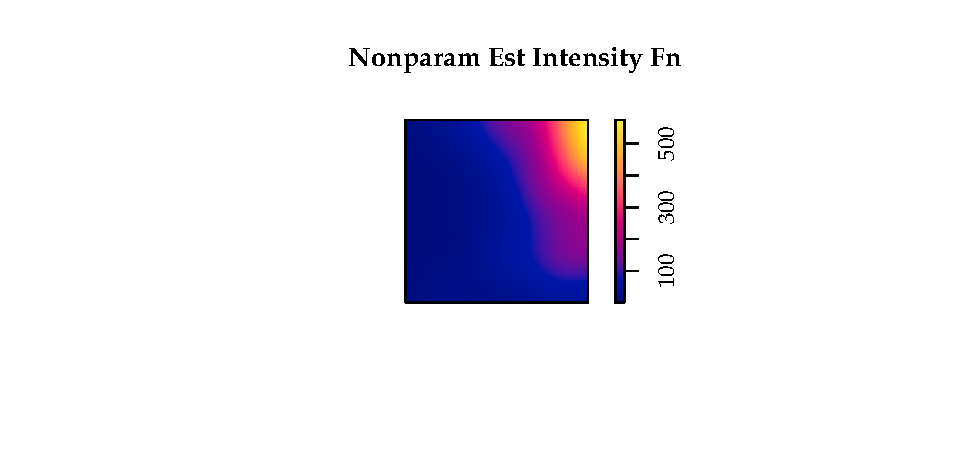
\includegraphics[width=\maxwidth]{figure/prob2f-1} 

}


\begin{kframe}\begin{verbatim}
Model diagnostics (raw residuals)
Diagnostics available:
	smoothed residual field
range of smoothed field =  [-46.09, 37.24]
\end{verbatim}
\end{kframe}
\end{knitrout}



\end{enumerate}

\item %3

{\it Recall the use of the nncorr statistic in the Finland Pines data set. The distribution of heights (the marks) was of interest. We saw that the nearest neighbor correlation between heights was  0.1839798. We questioned whether or not this was unusual. Carry out a randomization test to assess this. You can use the rlabel command to scramble the marks if you want. Provide me with a histogram of the randomization distribution and a p-value. Discuss BRIEFLY your results. Provide me with your R-code, also. (Note - you need to extract the correlation from the nncorr output. Here is how to do that:
}
\begin{knitrout}\footnotesize
\definecolor{shadecolor}{rgb}{0.969, 0.969, 0.969}\color{fgcolor}

{\centering 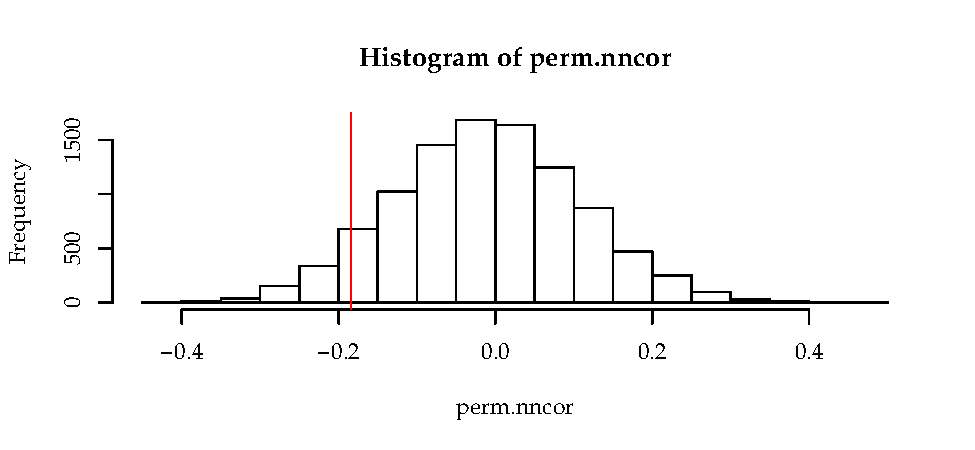
\includegraphics[width=\maxwidth]{figure/prob3-1} 

}



\end{knitrout}

$H_{0}:$ Pearson correlation = 0

$H_{a}$: Pearson correlation $\neq$ 0

The observed Pearson correlation between the nearest neighbor distance and the height was -0.184. A permutation test based on 10000 permutations of height led to a two sided p-value of 0.1207 which provides no evidence of a structured distribution of heights. Discussion with subject matter experts prior to data analysis may have lead to a one sided p-value.


\item %4

{\it Let’s derive a K function for something other than a CSR process. We will assume a Neyman- Scott process with the following properties.
i The parent process is a homogeneous Poisson process with intensity  .
ii The number of off pring produced by each parent (N) is homogeneous Poisson with
intensity $\mu$.
iii The position of each o↵spring is determined by a bivariate normal distribution with mean (0,0) (i.e. it is centered over the parent) and variance-covariance matrix  2I. Note that this implies that the x and y coordinates are determined independently of one another with the same variance.
}

See attached.
\end{enumerate}

\end{document}

